\documentclass[review,authoryear]{elsarticle}

\usepackage[T1]{fontenc}
\usepackage{textcomp}
\usepackage{color}
\usepackage[vlined,ruled]{algorithm2e}
\usepackage{array}
\usepackage{multirow}
\usepackage{booktabs}
\usepackage[table]{xcolor}

\usepackage{booktabs}
\definecolor{lightgray}{gray}{0.9}

\begin{document}

\begin{table}
\centering
\begin{tabular}{lcccccc}
\toprule
& Visual & Motor & dorsal attentive & salience & executive control & DMN \\
\cline{2-7}
K-Means & 195  & 251 & 378 &  253 & 563 & 469\\
\cline{2-7}
HMRF & 170 &  412 & 199 & 289 & 743 & 352 \\
\cline{2-7}
 Diff. &  -0.61 \%  & +2.19\%  & -2.68\%        &  +1.01 \%& +2.07\% &  1.41\%  \\

\bottomrule
\end{tabular}
\caption{To test the correlation of the network label maps and the age variable,
  a logistic regression test is performed on each voxels with age as independent
  variable, and the binary network label as response variable. The Wald test is
  used to test whether there exists significant correlation. After a FDR
  correction, no voxel's coefficient is significantly different from zero at
  $\alpha = 0.05$ level. This table shows the number of significant voxels
  without FDR correction for the functional networks estimated from a
  non-hierarchical model (K-Means) and our HMRF model. The bottom row shows the
  percentage of change in the total number of voxels that has been tested in a
  functional network. }
\end{table}



\begin{table}
\centering
\begin{tabular}{llcccccc}
\toprule
& & Visual & Motor & dorsal attentive & salience & executive control & DMN \\
\cline{2-8}
\multirow{2}{*}{$\chi^2$} & K-Means & 47 & 65 & 138 & 51 & 127 & 148\\
\cline{3-8}
& HMRF & 165 & 68 & 58 & 70 & 151 &  185 \\
& diff & +2.29\% & -0.04\% & +1.25\% & +0.53\% & 2.75\% & 0.44\% \\

\cline{1-8}
\multirow{2}{*}{Fisher's Exact} & K-Means & 79 & 333 & 164 & 74 & 96 & 79\\
\cline{3-8}
& HMRF & 106 & 126 & 112 & 134 & 227 & 106 \\
& diff & +0.66\% & 0.03\% & -0.01\% & 1.68\% & 1.50\% & 0.32\% \\
\bottomrule
\end{tabular}
\caption{To test the correlation of the network label maps and the sex
  categorical variable, we build a contingency table on each voxel with rows as
  sex and column as network labels. Then we use both $\chi^2$ test and Fisher's
  exact test to verify whether the functional network labels are independent of
  sex.  For both the non-hierarchical version of network estimation method
  (K-Means) and our HMRF method, no voxel's coefficient is significantly
  different from zero at $\alpha = 0.05$ level after a FDR correction. This
  table shows the number of significant voxels without FDR correction for the
  functional networks estimated from two methods. The bottom row shows the
  percentage of change in the total number of voxels that has been tested in a
  network. }
\end{table}

%% \begin{figure}
%% \includegraphics[width=1.0\textwidth]{figures/corr/corr}
%% \caption{The correlation map of the major functional networks estimated by the
%%   seed-based correlation analysis on the rs-fMRI data being spatially smoothed
%%   wtih 6mm FWHM. Seed regions are selected based on the work of
%%   \citet{van2010intrinsic} and \citet{seeley2007dissociable}. Seed coordinates
%%   are: Visual, (30, -88, 0), (-30, -88, 0); Motor, (-36, -25, 57), (36, 25, 57);
%%   attentive, (-24, -58, 52), (22, -58, 54); Salience, (18, 48, 26), (42, 48,
%%   26), (30, 48, 34); Executive control, (30, 51, 39); DMN, (0, -53, -26), (0,
%%   52, -6). One correlation map is estimated from each subject and each seed
%%   region. all the maps are averaged and thresholded at 0.05. }
%% \end{figure}

\begin{figure}
\includegraphics[width=1.0\textwidth]{figures/17networks/grp_mean}
\caption{The mean functional maps of the group over all bootstrapped rs-fMRI
  samples, with number of network set to 17. The binary maps of each network are
  averaged over all bootstarp samples.}
\end{figure}

\begin{figure}
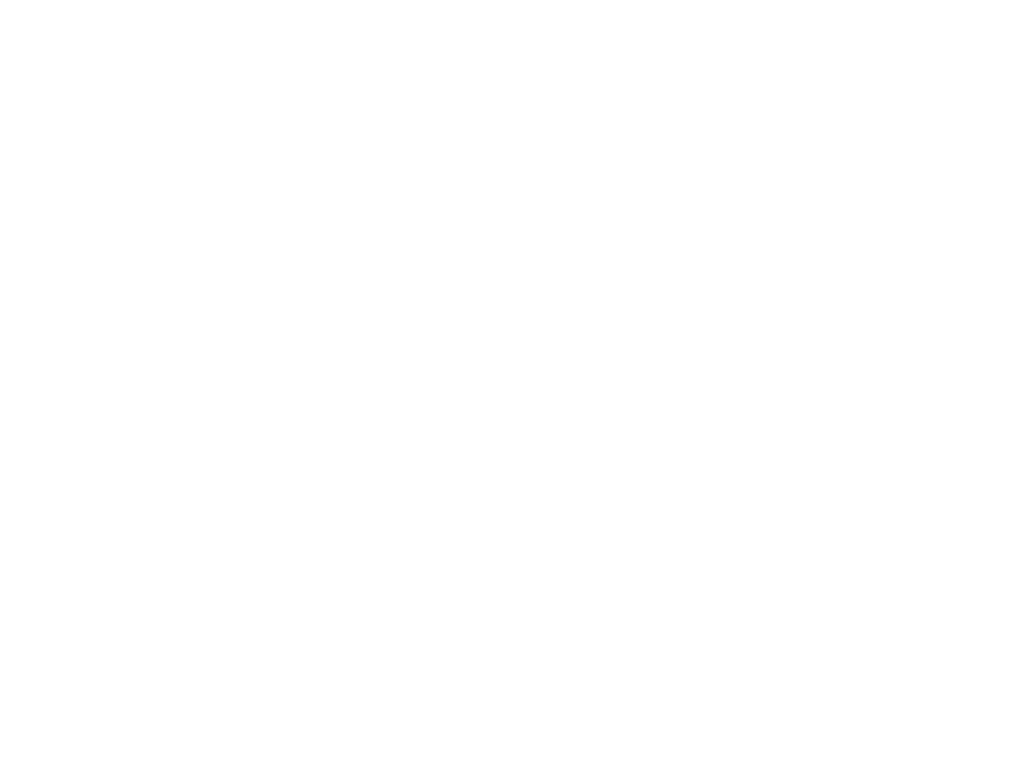
\includegraphics[width=1.0\textwidth]{figures/17networks/grp_var}
\caption{The group variance map estimated from all bootstrap samples, with the
  number of networks set to 17. The variance values range from 0.05 to 0.15. }
\end{figure}

\begin{figure}
\includegraphics[width=1.0\textwidth]{figures/17networks/sub_mean}
\caption{The mean functional maps of two subjects over all bootstrapped rs-fMRI
  samples, with number of network set to 17. The binary maps of each network are
  averaged over all bootstarp samples.}
\end{figure}

\begin{figure}
\includegraphics[width=1.0\textwidth]{figures/17networks/sub_var}
\caption{The subject variance map estimated from all bootstrap sample, with the
  number of networks set to 17. The variance values range from 0.05 to 0.15. }
\end{figure}

\begin{figure}
\includegraphics[width=1.0\textwidth]{figures/corr_overlay/corr_overlay_thick}
\caption{The correlation maps of the major functional networks estimated by the
  seed-based correlation analysis on the rs-fMRI data being spatially smoothed
  wtih 6mm FWHM. Seed regions are selected from \citet{van2010intrinsic} and
  \citet{seeley2007dissociable}. Seed coordinates are: Visual, (30, -88, 0),
  (-30, -88, 0); Motor, (-36, -25, 57), (36, 25, 57); attentive, (-24, -58, 52),
  (22, -58, 54); Salience, (18, 48, 26), (42, 48, 26), (30, 48, 34); Executive
  Control, (30, 51, 39); DMN, (0, -53, -26), (0, 52, -6). One correlation map is
  estimated from each subject, averaged over seeds, and threshold at 0.05. The
  network clusters identified by the proposed HMRF method, outlined with dark
  black lines, are overlaid on the corresponding correlation maps. For some
  networks, such as visual, motor, and DMN, the correlation maps and the HMRF
  clusters match well. For dorsal attentive, salience, and executive control
  that have larger intersubject variations, the clusters from HMRF look more
  like those of the group compared with the subject specific correlation
  maps. Some thicker area on the HMRF cluster outlines is due to the projection of
  3D surface on 2D slice. }

\end{figure}

\bibliographystyle{model2-names}
\bibliography{../myreference}
\end{document}
